\documentclass[12pt,a4paper,twoside,openright]{report}
\usepackage{algpseudocode}		% ambienti per la scrittura di algoritmi
\usepackage{algorithm}			% 

\usepackage{epsfig}						% figure eps
\usepackage{graphicx}					% figure qualsiasi
\usepackage{amsmath,amsfonts,amsthm}		% package di scrittura matematica
\usepackage{amssymb}
\usepackage{psfrag}
\usepackage{fancyhdr}
\usepackage{url}
\usepackage{array}
\usepackage{subfigure}
\usepackage{lscape}
\usepackage{colortbl}
\usepackage{alltt}
\usepackage{tabularx}
\usepackage[english]{babel}
\usepackage[nottoc]{tocbibind}
\sloppy
\raggedbottom

\linespread{1.3}
\renewcommand{\baselinestretch}{1.3}

\makeatletter
\def\cleardoublepage{\clearpage\if@twoside \ifodd\c@page\else
\hbox{}
\vspace*{\fill}
\begin{center}
%This page intentionally contains only this sentence.
\end{center}
\vspace{\fill}
\thispagestyle{empty}
\newpage
\if@twocolumn\hbox{}\newpage\fi\fi\fi}
\makeatother

%\newcites{wb}{Web References}

%------------------------------------------------------
% Impostazioni per il controllo sillabazione vedove/orfane ect..
%
% \looseness=1 o \looseness=-1 prima di un paragrafo per
% allungarlo o accorciarlo di una riga
%------------------------------------------------------

\lefthyphenmin=4
\righthyphenmin=4
\tolerance=1000
\hyphenpenalty=100
\emergencystretch=1 cm

\widowpenalty=5000
\clubpenalty=2500

%--------------------------------------------------------
% impostazioni per la dimensione delle pagine
%--------------------------------------------------------
\renewcommand{\headrulewidth}{0.5pt}
\hoffset=-15mm
%\topmargin=0mm
\headheight=15pt
\textwidth=140mm
\headsep=5mm
\voffset=-5mm
%\hsize=13cm
%\textwidth=164mm
\textheight=230mm
\evensidemargin=25mm
\oddsidemargin=25mm
%\marginparwidth=0mm

\renewcommand{\abovecaptionskip}{0pt}
\renewcommand{\belowcaptionskip}{0pt}

%--------------------------------------------------------------
%impostazione headers
%--------------------------------------------------------------
\pagestyle{fancy}
%\addtolength{\headwidth}{\marginparsep}
%\addtolength{\headwidth}{\marginparwidth}
\renewcommand{\chaptermark}[1]{\markboth{#1}{}}
\renewcommand{\sectionmark}[1]{\markright{\thesection\ #1}}
\fancyhf{}
\fancyfoot[LE,RO]{\bfseries\thepage}
\fancyhead[RO]{\bfseries\rightmark}
\fancyhead[LE]{\bfseries\leftmark}
\fancypagestyle{plain}{%
\fancyhead{} % get rid of headers
\fancyfoot{}
\renewcommand{\headrulewidth}{0pt} % and the line
}

\newenvironment{myverse}
{\small}
{}

\newenvironment{myabstract}{%
  \begin{center}%
    \null\vfil
    \bfseries \abstractname
  \end{center}}%
{\par\vfil\null}

%------------------------------------
\newcommand{\name}{$\mathcal{H}$eaven } 
\newcommand{\namens}{$\mathcal{H}$eaven} 
%------------------------------------
\begin{document}

\pagenumbering{roman}
\setcounter{page}{1}
\pagestyle{empty}

%--------------------------------------------------------------------------------
% include title page
%--------------------------------------------------------------------------------
%\linespread{1}
\begin{titlepage}
\vspace*{-2.5cm}
\bfseries
\begin{center}
  \LARGE
  Politecnico di Milano\\
  \Large
  School of Industrial and Information Engineering\\


\psfig{file=images/logopm,width=4cm}

\begin{large}
Department of Electronic, Informatics and Bioengineering\\
Engineering of Computer Systems\\
\end{large}

\vspace{1.0cm}
\begin{Large}
\namens: Supporting Systematic Comparative Research of RDF Stream Processing Engines
\end{Large}  
\end{center}
\vspace*{4.5cm}
\large
\begin{flushleft}
\hspace{-2cm}  Advisor: Emanuele DELLA VALLE\\
\hspace{-2cm}  Co-Advisor: Daniele DELL'AGLIO\\
\end{flushleft}
\vspace*{1.5cm}

\hspace{1.5cm}
\parbox{14cm}{
    \begin{tabular}{lll}
        Master thesis by: & Riccardo TOMMASINI    & matr. 799120\\
    \end{tabular}
}

\vspace*{1.4cm}
\begin{center}

  Academic Year 2013-2014



\end{center}
\end{titlepage}
\cleardoublepage

%--------------------------------------------------------------------------------
% dedica
%--------------------------------------------------------------------------------
\thispagestyle{empty}

\begin{flushright}
\large\textit{To Aldo\\ }
%\large\textit{I miss you\dots\\}
\large\textit{and to my family,\\ }
\large\textit{thanks for all your support (and the fish)\dots\\}


\end{flushright}

%\null\vfil

\cleardoublepage

%--------------------------------------------------------------------------------
% ringraziamenti
%--------------------------------------------------------------------------------
\thispagestyle{empty}

\chapter*{Acknowledgements}

\begin{flushleft}
Milano, 1 Aprile 2015
\end{flushleft}
Ringrazio il Professor Emanuele Della Valle, che ha reso la tesi un percorso incredibilmente formativo. \`E stato un lavoro impegnativo, ma sempre stimolante e divertente. Grazie per l'opportunit\`a, il tempo dedicatomi e l'infinita quantit\`a di suggerimenti ricevuti. Sono grato anche a Daniele Dell'Aglio, per la sua guida e l'aiuto tecnico e per aver reso stimolante ogni discussione. Un sentito ringraziamento anche a Marco Balduini, per il suo prezioso contributo, in un momento, per lui, sicuramente molto difficile.

Ringrazio la mia famiglia, per avermi sostenuto nelle piccole difficolt\`a quotidiane, che da solo non avrei mai potuto superare, e per avermi insegnato che vale sempre la pena impegnarsi al massimo.

Ringrazio gli amici della MTF, per non avermi permesso di abbandonarli del tutto e per aver condiviso momenti unici e di incredibile sincerit\`a.

Ringrazio Teto. Cinque anni fa abbiamo iniziato insieme questa corsa e, come uno di famiglia, ci sei stato fino alla fine.

Ringrazio Francesco, per tutte le discussioni assurde che abbiamo fatto, i consigli onesti e per essere un vero amico da pi\`u di dieci anni.

Ringrazio Fabiana, per essere stata una guida spirituale, per avermi motivato e per aver sciolto nodi che stanno nella mia testa e nel cuore, non solo nei muscoli. Ringrazio anche Alberto, perch\`e lavora sempre dietro le quinte.

Ringrazio i Bomber, Fabio e Lorenzo. Per avermi mostrato come ci si diverte lavorando; per avermi dimostrato che chi punta in alto arriva in alto e soprattutto per avermi insegnato che "Nobody Works Like Us". Che dire ragazzi, se non "\textit{we were stuck in a blender, and now we are saving lives. WHAT?}"

\begin{flushright}
\emph{Riccardo}
\end{flushright}

\cleardoublepage
\thispagestyle{empty}

\pagestyle{fancy}
\renewcommand{\contentsname}{Table of Contents}%

%--------------------------------------------------------------------------------
% include the abstract in italian
%--------------------------------------------------------------------------------
\chapter*{Estratto}
Lo Stream Reasoning \`e  il settore di ricerca che ha dimostrato la possiblit\`a di applicare procedure di reasoning su flussi informativi in rapido cambiamento. Un RDF Stream Processing (RSP) Engine \`e  un sistema in grado di processare a livello semantico questi flussi, quando sono codificati secondo lo standard RDF. Il numero di RSP Engine implementati \`e  in crescita e di conseguenza la comunit\`a scientifica sta formalizzando i metodi e gli strumenti che hanno consentito lo sviluppo di queste soluzioni.

Diversi settori di ricerca nell'ambito della Computer Science, hanno mostrato interesse per una maggiore comprensione della natura del proprio lavoro. Sono stati fatti diversi studi che hanno analizzato i frutti della ricerca in questi settori~\cite{Tichy:1995:EEC:209090.209093, Wainer:2009:EEC:1518331.1518552}. Questi hanno dimostrato anzitutto la natura ingegneristica di molte pubblicazioni nell'ambito della Computer Science, ma anche una discreta mancanza di valutazioni empiriche delle soluzioni implementate. Questa \`e  una differenza evidente con le altre aree di ricerca legate al mondo dell'ingegneria, che si focalizzano su questo tipo di analisi.

Solitamente, nei settori informatici in cui la valuazione empirica \`e tralasciata, i sistemi proposti hanno una natura complessa e sfaccettata che \`e difficile da valutare. Tuttavia \`e  possibile, con gli strumenti adatti, studiare anche casi complessi. Questo accade per le scienze sociali o l'economia, i cui soggetti d'indagine non sono di certo facilmente modellabili. In questi settori viene comunemente usato un approccio comparativo sistematico, che semplifica il problema di affrontare soggetti complessi, senza tralasciare gli aspetti che li rendono rilevanti. Questo approccio diventa applicabile solo in un contesto sperimentale appropriato, che garantisce propriet\`a come riproducibilit\`a, ripetibilt\`a e comparabilit\`a.

La comunit\`a dello Stream Reasoning ha colto la necessit\`a di fornire strumenti per valuare correttaemente gli RSP Engine,  comprenderne il comportamento e quantificarne il valore comparando le prestazioni in casi d'uso reali. Qualche passo in questa direzione \`e  stato gi\`a fatto. Lavori recenti~\cite{Zhang2012, LePhuoc2012c, DBLP:conf/semweb/DellAglioCBCV13} hanno fornito framework di benchmarking per RSP Engine, mentre altri hanno posto le basi di queste valutazioni~\cite{DBLP:conf/esws/ScharrenbachUMVB13}, mostrando quali erano le mancanze di tali framework.

Le soluzioni proposte si sono dimostrate limitate, e la valutazione empirica di RSP Engine \`e  solo all'inizio. Quello che ancora manca \`e  una infrastruttura che permetta la comparazione sistematica di RSP Engine, all'interno di un contesto sperimentale che goda delle proprit\`a sopracitate. Per affrontare il problema, in questa tesi, abbiamo preso dall'ingegneria aerospaziale l'idea di un banco di prova, uno strumento di valutatione e sviluppo per motori.

Un banco di prova permette di progettare esperimenti ed eseguirli su qualsiasi motore, raccogliendo i dati per una successiva valutazione delle prestazioni. %Dal punto di vista scientifico un esperimento gode di tre proprit\`a fondamnetali: riproducibilit\`a, ripetibilit\`a e comparabilit\`a, tre pilastri su cui \`e  possible costrurie un approccio comparativo sistematico per la ricerca. 
La nostra domanda di ricerca quindi \`e : "Un banco di lavoro per RSP Engine \`e  la soluzione che permetta la ricerca comparativa e sistematica nell'ambito dello Stream Reasoning?"

In questa tesi proponiamo \namens, un framework open source per la ricerca comparativa e sistematica nell'ambito dello Stream Reasoning. Il framework si compone di un Banco di Lavoro, l'equivalente di quanto abbiamo visto nell'ingegneria aerospaziale ma per RSP Engine. Include quattro implementazioni naive di RSP Engine, dette Baselines. Questi sistemi semplificati permettono di iniziare la ricerca comparativa. Infine \name contiene l'Analyser, un insieme di metodi di indagine e strumenti di supporto, organizzati gerarchicamente ed atti ad analizzare e comparare i dati raccolti attraverso l'esecuzione di esperimenti su RSP Engine tramite il banco di lavoro.


%--------------------------------------------------------------------------------
% include the abstract in english
%--------------------------------------------------------------------------------
\chapter*{Abstract}
Stream Reasoning research field is grown enough to prove that reasoning upon rapidly changing information is possible. The number of implemented RDF Stream Processing (RSP) Engine, systems capable to handle at semantic level RDF-encoded information flows, is increasing. Now the Stream Reasoning community is working on the standardisation of the methods and tools that supported the development of those solutions. Moreover, it is mandatory to provide an evaluation of RSP Engines, which allows to understand how these systems perform in real uses cases. 
Recent works in the filed \cite{Zhang2012, LePhuoc2012c, DBLP:conf/semweb/DellAglioCBCV13} pursued this goal, providing many benchmarks for evaluating RSP Engines. Further analysis of RSP Engines \cite{DBLP:conf/esws/ScharrenbachUMVB13} pointed out the challenges involved by the Stream Reasoning research. \cite{DBLP:conf/esws/ScharrenbachUMVB13} posed the basis for a proper evaluation of such a system, describing in detail where these works have failed and where the can be improved.

In parallel, many  Computer Science (CS) research fields tried to understand the nature of their own research. The related studies \cite{Tichy:1995:EEC:209090.209093, Wainer:2009:EEC:1518331.1518552} shown the affinity of many CS research fields to an Engineering epistemology. But they also evinced and criticised the concrete differences with other engineering research areas, which focus on evaluation of the proposed systems and not only on their design and development. The lacks of an empirical approach can be ascribed to the complex nature of the software systems. However, it is possible to face complex case studies which are not be easily modelled. Social science and economy researchers found methods to deal with them.

The Stream Reasoning research suffers from the same lack. The limitations of the existing benchmarking proposals proved that the empirical evaluation of RSP Engines is just at the beginning. What is still missing in an infrastructure that allows to compare, maybe automatically, the performances of many RSP Engines. We borrow from the aerospace engineering the idea of an engine test stand, which is an automatic facility for engine testing. A test stand allows to design experiments and to execute them, evaluating engines in a controlled environment. %Experiment properties like reproducibility, repeatability and comparability represent the pillars upon which we can start the empirical evaluation of RSP Engines.
Thus, we formulate the following research question: "\textit{Can an engine test stand, together with queries, datasets and methods, support Systematic Comparative Research Approach for Stream Reasoning?}"

In this thesis we propose \namens, an open source framework that enables the Systematic Comparative Approach in the Stream Reasoning research field. \name consists in:  an RSP Engine Test Stand, which emulates the aerospace engineering facility in the Stream Reasoning context; the Analyser, which enables the Systematic Comparative Approach trough a set of methods and tools for the investigation, hierarchically organised into an stack; and, finally, four naive implementations of RSP Engines, called Baselines, which represent simple terms of comparison upon which  start the comparative research.

%--------------------------------------------------------------------------------
% talbe of contents
%--------------------------------------------------------------------------------
\tableofcontents
\cleardoublepage

\pagenumbering{arabic}

\setcounter{page}{1}


%--------------------------------------------------------------------------------
% introduction
%--------------------------------------------------------------------------------
\chapter{Introduction}
\label{chap:one}
Introduzione al lavoro. Inizia direttamente, senza nessuna sezione.

Argomenti trattati suddivisi sezione per sezione\dots

Per citare un articolo, ad esempio \cite{Ackley1987} o \cite{Ackley1987,Altenberg1994} utilizzare il comando \texttt{\\cite}. 

Per gestire i file di tipo \texttt{bib} esiste il programma \texttt{JabRef} disponibile sul sito \texttt{http://jabref.sourceforge.net/}.

\section*{Original Contributions}
This work include the following original contributions:
\begin{itemize}
\item \dots riassunto sintetico dei diversi contributi
\item \dots
\item \dots
\end{itemize}

\section*{Outline of the Thesis}
This thesis is organized as follows: 
\begin{itemize}
\item In Chapter~\ref{chap:one} \dots
\item In Chapter~\ref{chap:two} \dots
\item In Chapter~\ref{chap:three} \dots
\item \dots
\end{itemize}
Finally, in Chapter~\ref{chap:conclusions}, \dots




%--------------------------------------------------------------------------------
% chapters
%--------------------------------------------------------------------------------
\chapter{\dots}
\label{chap:two}
\section{Introduction}
Introduzione agli argomenti trattati nel capitolo, dalle 4 alle 10 righe.

\section{\dots}
Argomenti trattati suddivisi sezione per sezione\dots

\section{Figure}
Per includere delle figure come la Figura~\ref{fig:figura} 
usare il comando \texttt{\\includegraphics}.

%--------------------------------------------------------------------------------
% esempio di inclusione immagine
%--------------------------------------------------------------------------------
\begin{figure}[tbh]
  \centering
  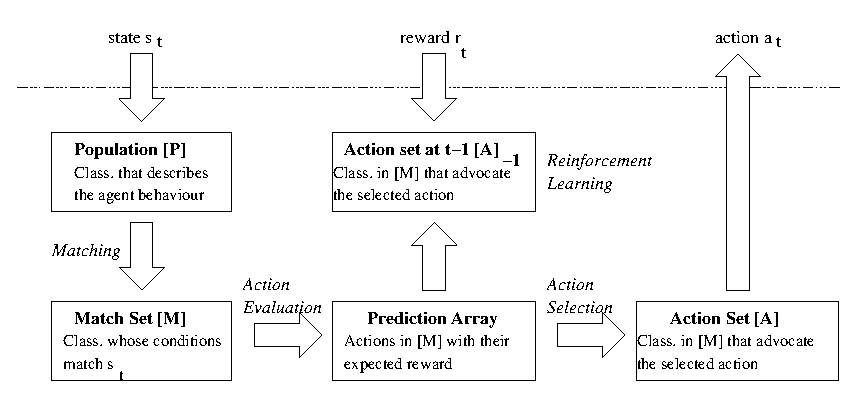
\includegraphics[scale=0.7]{images/esempio}
  \caption{\dots titolo}
  \label{fig:figura}
\end{figure}

\section{Algoritmi}
Per includere degli algoritmi come l'Algoritmo~\ref{alg:esempio}
usare lo stile \texttt{algpseudocode} presente nel package~\texttt{algorithmicx}.

%--------------------------------------------------------------------------------
% esempio di algoritmo
%--------------------------------------------------------------------------------
\begin{algorithm}[t]
  %%%
%%%
%%%	the Q-learning algorithm
%%%
%%%
\begin{algorithmic}[1]
\State Initialize $Q(\cdot,\cdot)$ arbitrarily
\ForAll{episodes}
   \State $t$ $\leftarrow$ 0
   \State Initialize $s_{t}$
   \Repeat
      \State $a_{t} \gets \pi(s_{t})$
      \State perform action $a_{t}$; observe $r_{t+1}$ and $s_{t+1}$
      \State $Q(s_{t},a_{t}) \gets Q(s_t,a_t) + \alpha( r_{t+1} + \gamma \max_{a\in A} Q(s_{t+1},a) -  Q(s_t,a_t))$
      \State $t \gets t+1$
   \Until{$s_{t}$ is terminal}
\EndFor
\end{algorithmic}

  \caption{Un esempio di algoritmo.}
  \label{alg:esempio}
\end{algorithm}


\section{Summary}

Riassunto del capitolo

%--------------------------------------------------------------------------------
% problem settings
%--------------------------------------------------------------------------------
\chapter{Problem Settings}
\label{chap:ps}
In this Chapter we introduce the work this thesis involved. First we introduce the motivations behind this research. In Section \ref{sec:comparative-research} we describe the themes that have inspired this survey towards the Comparative Research and, as a conclusion, we formulate our research question. Then, in Section \ref{sec:requirements} we formalise the requirements we have to satisfy in order to successfully answer the research question.

\section{Comparative Research}\label{sec:comparative-research}
The Computer Science (CS) community classifies its activity in many works and shows that its research mostly follow an engineering epistemology \cite{Wainer:2009:EEC:1518331.1518552,Tichy:1995:EEC:209090.209093}. A majority of publications belongs to \textit{empirical work} and \textit{design \& modelling} classes of Tichy's taxonomy (See \ref{sec:tcp} ) and, among them, proposals of new systems or models  are more common then the evaluations of existing ones. This contrasts with other engineering areas, where the experimental research is almost dominant. CS needs to focus on collecting, analysing, and interpreting the observations of those works it usually only designs or implements. Now the question is: \textit{What are the motivation under this CS research lack?} The main problem in evaluating software systems or models regards their complex and multifaceted nature. Other explanations concern the difficulties of conducting realistic evaluations, because of the number of the involved variables.

A Systematic Comparative Research Approach (SCRA) is typically used in those research fields where the complexity of its research subjects goes beyond the possible observable models. This is the case of the social sciences, which exploit techniques to deal with complex cases that can not be simplified in experimental setting. The analysis of a single case study allows to deeply understand it, but it makes difficult to engage any form of generalisation. On the other hand, cross-case studies are more relevant and allow general thinking, but their final complexity represents a problem. We need a strategy that reduces the analysis complexity without lose the relevance of each involved system. In this regard, Russel Schutt discusses four stages to systematic qualitative comparative studies for history social phenomena:
\begin{enumerate}
\item[S.1] Premise of the investigation: identification of possible causes.
\item[S.2] Choose the cases to examine (location, language, gender).
\item[S.3] Examine the similarities and the differences with shared methods.
\item[S.4] Propose a causal explanation for the phenomena.
\end{enumerate} We will return on these stages later. Is important to understand that this investigation method becomes meaningful inside the experimental environment. An \textit{experiment} is a test under controlled conditions that is made to demonstrate a known truth or examine the validity of an hypothesis (W.R Inge). Complex cases are seen as a combination of known properties upon which is possible to identify parallelism or state contrasts and are used to set up experiment configuration. Researcher can exploit the notions of \textit{reproducibility} to appreciate variations on changing experiment conditions, \textit{repeatability} to consolidate observations trough multiple identical executions and \textit{comparability} to contrast the results to identify the differences.

Some Computer Science sub-fields attempt to lead Case-driven analysis by the notion of experiment. Database community explores the idea of comparative research trough benchmarking techniques and actually the quality of empirical studies is rising \cite{Wainer:2009:EEC:1518331.1518552}. It is worth to note Jim Gray's work about transactional benchmarking (TCP, Section \ref{sec:tcp}) and Domain Specific Benchmarks (DSB). He states that \textit{any comparison on performances starts with the definition of a benchmark or a workload}, but we need know the relevance of the metrics. Measurement variations are very frequent from one application to another, because each system is thought to solve a small problems set. A DSB must response properly to system diversities, by specifying a synthetic workload to describe typical applications in the problem domain; moreover it must provide workload performances on various systems and an estimation of relative performance on the problem domain.
Gray proposes also four criteria that a DSB must meet, which are:
\begin{enumerate}
\item[G.1] \textsc{Relevance}, it must measure the performance peak of systems when
performing domain typical operations.
\item[G.2] \textsc{Portability}, it must be easy-to-implement on many different systems and architectures
\item[G.3] \textsc{Scalability}, it must be meaningful for both small and large computer systems
\item[G.4] \textsc{Simplicity}, it must be understandable to obtain credibility
\end{enumerate} 

Let's consider the relation between this criteria and Schutt's stages presented above. Gray states G.1 to identify the relevant metrics for the evaluation, as Schutt does in his first stage (S.1), which demands a pre-analysis phase of the phenomenon. Moreover, Social Science does not care about problem scaling, because those properties that define the case also determine the problem dimension (S.2). Gray poses the same concept in the DB context with G.2, demanding implementation-related conditions, but it also explicit the need to consider the dimension-related issues in G.3, because DB must consider the scaling problem. Last but not least, G.4 demands simplicity to obtain credibility while S.3 suggests to exploit those evaluation methods that are commonly accepted (shared) by the research community. 

Motivated by the growing number of RDF Stream Processing techniques, the Stream Reasoning (SR) community strongly calls of evaluation practices to allow comparison on them. RSP Engines, the systems that implement this techniques, have an high resulting complexity (Further details in Section \ref{sec:sfp}). The execution mechanism they implement together with their execution semantic and the environment where this execution happens are evaluation-related characteristics, which demonstrate that a meaningful comparison between RSP Engines is non-trivial. Chapter 	\ref{chap:evaluation} shows in details that may be difficult to analyse those system, even in case of simple and well defined architectures. 
The interest on cross-case analysis between complex subjects draw the need of a comparative research approach. Initial efforts in this direction try to define frameworks that resume  DSMSs \cite{arasu2004linear} and Reasoning \cite{Guo2005} benchmarking studies. LS Bench and SR Bench propose a set of queries, data sets, and methods to test and compare existing RSP engines (see Section\ref{sec:sr-benchmarking}). Both these works share a common background: the Linear Road Benchmark (LRB) is the only existing benchmark for relational data stream processing engines. Actually LRB only states which requirements a benchmarked DSMS must satisfy, without proposing a concrete solution. LS Bench and SR Bench implement and extend this work, but they do not re-contextualise this requirements in SR context. Following discussions identify other lacks, i.e none of them completely face the problem of evaluating query result correctness, because they do not analyse engine semantics. LS Bench concentrates attention to the evaluation of engines throughput and it checks the correctness of the query result measuring the mismatch after comparing different RSP Engines. SR Bench entirely ignores this issue and analyses the coverage of SPARQL constructs for each commercial engine. More recent works describe deeply all the RSP Engine properties, identify the future challenges and provide a standardization benchmarking requirements: commandments for a meaningful testing on RSP Engines\cite{DBLP:conf/esws/ScharrenbachUMVB13}.

Stream Reasoning community still lacks an infrastructure that can control the execution environment and allow to systematic testing. LRB provides a simulator to validate the benchmarked DSMS systems, but does not face the problem of an online evaluation it. Researches in this area demonstrates that RSPEngine execution semantic is relevant \cite{Botan:2010:SMA:1920841.1920874}, but does not evaluate its cost. From the aerospace engineering we borrow the idea of an \textit{Engine Test Stand}, a tool that allows experiments design, their systematic execution and automatic results comparison. An engine can not be evaluated only by an architectural viewpoint, it is necessary to understand it behaviour during the execution: \textit{A process cannot be understood by stopping it. Understanding must move with the flow of the process, must join it and flow with it}\footnote{The First Law of Mentat, quoted by Paul Atreides to Reverend Mother Gaius Helen Mohiam}. Thus, the community questioned itself \textit{How to support SRCA on RSP Engines}? Now we have queries, dataset and methods, that partially answer it and the new research question is "\textit{Can an engine test stand, together with queries, datasets and methods, support SCRA for Stream Reasoning?}". The next section poses the requirements a proper answer to this research question must satisfy.

\section{Requirements} \label{sec:requirements}

In order to simplify and support Systematic Comparative Research Approach on RSP engines trough an Engine Test Stand we need to answer the following questions: 
\begin{enumerate}
\item[Q.1] How can the behaviour of system be evaluated? 
\item[Q.2] What makes this evaluation rigorous? 
\item[Q.3] How can this rigorous evaluation be automated?
\end{enumerate} To answer Question Q.1 we exploit traditional definition of \textit{experiment} presented above. We answer Q.2 referring to \textit{reproducibility}, \textit{repeatability}, and \textit{comparability} of experiments. Trough this concepts it is easy to answer Q.3 formalising the requirements for the solution.

\textit{Reproducibility} refers to measurement variations on a subject under changing conditions. We gather this conditions into experiment configuration, whose specification is up to the user. For this reason the solution must be independent from:
\begin{enumerate}
\item[R.1] \textit{Test data}, relevant RDF data streams and ontologies chosen from user domain of interest. %R.2.1
\item[R.2] \textit{Query}, relevant queries registered from user domain of interest.
%thus allowing users to register relevant queries from their domains of interest. %R.2.2
\item[R.3] \textit{Engine}, any RSP Engine tested by the means of easy-to-implement software interfaces. 
%thus allowing users to put an RSP engine on the test stand by the means of easy to implement software interfaces, e.g., it should adopt an event-base architecture as normally done by RSP engines and present events to RSP engine in a simple to parse RDF serialisation. %R4 e R5
\end{enumerate}

\textit{Repeatability} refers to variations on repeated measurements on a subject under identical conditions. The solution must not affect the RSP engine evaluation, which, from a practical point of view, poses two requirements:
\begin{enumerate}
\item[R.4] it must not be running when the RSP engine is under execution. %R.1.2
\item[R.5] it must have reduced (and possibly constant) memory footprint. %R.1.1
\end{enumerate}

\textit{Comparability} refers to performance measurements nature and the relations between experimental conditions. The SCRA demands both the definition of \textit{comparable metrics} and the standardization of \textit{evaluation methods}, which means the solution must:
\begin{enumerate}
\item[R.6] include \textit{basic set of performance measurements} \cite{DBLP:conf/esws/ScharrenbachUMVB13}.
\item[R.7] enable users extensions with new software sensors and specific measurements collection.
%\item[R.7] enable users software extensionsa and specific measurements collection.
\item[R.8] support performance measurements collection for further analysis.
\item[R.9] allow \textit{qualitative analysis} trough tools for result visualization
\end{enumerate}


In terms of software engineering, any solution which satisfies the requirements above demands also some technical ones: 
\begin{enumerate}
\item[R.10] \textit{Extendible Design}, the possibility to replace theoretically each module with one with the same interfaces, but different behaviour, without affecting architecture stability.
\item[R.11] \textit{Event-base architecture} to properly communicate with  RSP Engines, which normally exploit it.
\item[R.12] \textit{Easy-to-Parse RDF Serialisation} for the events presented to the RSP Engine in exam
\end{enumerate}

SCRA is case-oriented, it needs \textit{successful analysis and evaluations examples} to pose experimental guidelines and \textit{initial terms of comparison}. We call baseline an elementary solution for the RSP problem, which is relevant from an experimental viewpoint. To fulfil this request the answer to our research question must consider to have specific baseline modules and satisfy their own requirements, which are: \begin{enumerate}
%\item[R.13] Be a Solution: it solves the problem entirely, without concerning about performance. % devono risolvere interamente il problema, nel nostro caso devono essere complete e sound rispetto ad entailment regime che si è scelto
\item[R.13] It must be Elementary: requiring the minimum design effort, which means be a naive solution and do not care about performances.  % non devono essere soluzioni smart, devono chiedere il minimo effort
\item[R.14] It must be Eligible: being a fair term of comparison w.r.t. commercial solutions. %e' inutile se sono sopra un'ordine di grandezzaad esempio in latenza, rispetto ad una soluzione commerciale. probabilmente è sbagliata la domanda di ricerca
\item[R.15] It must be Relevant: covering one of the theoretical solutions. %la soluzione che coprono deve essere una delle immediate soluzioni del problema iniziale: Graph vs Statement o Inc vs Naive, tempo controllato esternamente, ecc
\item[R.16] It must be Simple: allowing to identify easily those characteristics which support hypothesis formulation and comparison.  %non devono offrire api più complesse rispetto a un RSPEngine tradizion	ale.
\end{enumerate}

%Some of those requirements assume a problem-specific meaning. As advocated in the early works on Stream Reasoning \cite{1,2} the most simple approach to create a stream reasoning system is arrange into a pipeline DSMS with a reasoner. Baselines design must follow this statement to develop a full solution [R.13] which is very simple w.r.t the commercial ones presented in Chapter 2 [R.14]. Chapter 2 also states how two main design decisions can distinguish the baselines: the RDF stream model and the architecture. From this point of view the solution must provide at least four Baselines [R.16], which cover all possible combinations those design choices.


%--------------------------------------------------------------------------------
% conclusions and future works
%--------------------------------------------------------------------------------
\chapter{Conclusions and Future Works}
\label{chap:conclusions}
Conclusioni del lavoro e sviluppi futuri. Massimo una o due pagine.

%--------------------------------------------------------------------------------
% appendices
%--------------------------------------------------------------------------------
\part*{Appendices\label{part:app}\addcontentsline{toc}{part}{Appendices}}
\appendix
\chapter{\dots}
\label{app:one}
\section{Introduction}
Introduzione agli argomenti trattati nell'appendice, dalle 4 alle 10 righe.

\section{\dots}
Argomenti trattati suddivisi sezione per sezione. 
Alla fine del capitolo non includere alcun sommario.



\chapter{\dots}
\label{app:two}
\section{Introduction}
Introduzione agli argomenti trattati nell'appendice, dalle 4 alle 10 righe.

\section{\dots}
Argomenti trattati suddivisi sezione per sezione. 
Alla fine del capitolo non includere alcun sommario.


\bibliographystyle{plain}
\bibliography{tesi.bib}
\end{document}
